% Hanzo Base: The Single-Binary Runtime for Sovereign Applications
\documentclass[11pt]{article}
\usepackage{shared/hanzocover}
\usepackage{amsmath, amssymb, amsthm}
\usepackage{mathtools}
\usepackage{bm}
\usepackage{graphicx}
\usepackage{booktabs}
\usepackage{hyperref}
\usepackage{enumitem}
\usepackage{xcolor}
\usepackage{float}
\usepackage{multirow}
\usepackage{listings}
\input{shared/lstlang}
\usepackage{tikz}
\usetikzlibrary{shapes,arrows,positioning,fit}
\usepackage{pgfplots}
\pgfplotsset{compat=1.18}

\hypersetup{colorlinks=true,linkcolor=black,citecolor=blue,urlcolor=blue}

\definecolor{codegreen}{rgb}{0,0.6,0}
\definecolor{codegray}{rgb}{0.5,0.5,0.5}
\definecolor{codepurple}{rgb}{0.58,0,0.82}
\definecolor{backcolour}{rgb}{0.95,0.95,0.92}

\lstdefinestyle{mystyle}{
    backgroundcolor=\color{backcolour},
    commentstyle=\color{codegreen},
    keywordstyle=\color{codepurple},
    numberstyle=\tiny\color{codegray},
    stringstyle=\color{codegreen},
    basicstyle=\ttfamily\footnotesize,
    breakatwhitespace=false,
    breaklines=true,
    captionpos=b,
    keepspaces=true,
    numbers=left,
    numbersep=5pt,
    showspaces=false,
    showstringspaces=false,
    showtabs=false,
    tabsize=2
}
\lstset{style=mystyle}

\newtheorem{definition}{Definition}

\title{HANZO BASE\\[0.3em]
{\large The Single-Binary Runtime for\\Sovereign Applications}}
\author{
    Zach Kelling \\
    \textit{Hanzo Industries Inc (Techstars '17)} \\
    \texttt{research@hanzo.ai}
}
\date{March 2026}

\begin{document}
\hanzocoverpage

% ============================================================================
% ABSTRACT
% ============================================================================
\begin{abstract}
We present Hanzo Base, the application runtime for sovereign software. Base is
not a backend framework. It is the personal computer of Web5---a single Go
binary that packages an encrypted embedded database (SQLite with sqlcipher), a
realtime API layer, CRDT-based collaboration, a JavaScript plugin runtime
(Goja VM), Hanzo IAM authentication, and field-level KMS encryption into one
process. Where Firebase assumes a cloud provider, Supabase assumes PostgreSQL,
and PocketBase assumes a single user, Base assumes nothing. It runs on a
laptop, a phone, a Raspberry Pi, or a Kubernetes pod with the same binary and
the same API surface. Data stays local by default. Replication is opt-in.
Chain anchoring is available but never required. We describe the architecture,
the data plane (local vault, provider-optional replication, Lux receipt
anchoring), Base Functions (TypeScript in Goja, event-driven, zero cold start),
Base Collections (schemaless records with access rules and field-level
encryption), Base Sync (CRDT log, conflict-free merge, offline-first,
peer-to-peer or server-relay), and integration with Lux Network
chains (K-Chain key policy, I-Chain identity, T-Chain threshold controls).
Benchmarks on an M4 MacBook show 10,400 writes/sec for encrypted collections
and sub-millisecond read latency. In production since December 2022, Base
serves as the default runtime for 2,800+ applications across the Hanzo
ecosystem.
\end{abstract}

% ============================================================================
\section{Introduction}
\label{sec:intro}
% ============================================================================

Software is not sovereign. The applications people depend on daily---messaging,
notes, banking, health records---exist as tenants on infrastructure controlled
by third parties. The user's data lives in a provider's database, encrypted
with the provider's keys, governed by the provider's terms. If the provider
disappears, so does the application. If the provider changes policy, the user
complies or loses access. This is not ownership. It is tenancy.

The problem is architectural. Cloud-native design treats the network as a given:
every read is a round-trip, every write is a permission request, every query is
metered. The application is a thin client to someone else's computer. The
alternative---self-hosting---requires expertise that excludes all but a small
technical minority. There is no middle ground.

Base is the middle ground.

\begin{definition}[Sovereign Application]
An application is sovereign if: (i) the user controls the encryption keys for
all stored data, (ii) the application functions without any network connection,
(iii) replication to any remote host is opt-in and reversible, and (iv) no
third party can unilaterally revoke access to the application or its data.
\end{definition}

Base achieves sovereignty by inverting the cloud model. Instead of a thin
client talking to a remote server, Base is the server---running locally, owning
its own database, generating its own keys. Remote services (cloud storage, chain
anchoring, peer sync) are optional extensions, never requirements.

\subsection{Contributions}

\begin{enumerate}[leftmargin=1.4em]
    \item A single-binary application runtime with embedded encrypted database,
    realtime APIs, authentication, and plugin system
    (\S\ref{sec:architecture}).
    \item A data plane architecture where local storage is primary and remote
    replication is provider-optional (\S\ref{sec:dataplane}).
    \item Base Functions: TypeScript execution in an embedded Goja VM with
    zero cold start and event-driven hooks (\S\ref{sec:functions}).
    \item Base Collections: schemaless records with row-level access rules and
    field-level KMS encryption (\S\ref{sec:collections}).
    \item Base Sync: CRDT-based conflict-free replication supporting
    offline-first, peer-to-peer, and server-relay topologies
    (\S\ref{sec:sync}).
    \item Integration with Lux Network for key policy, identity, and threshold
    controls (\S\ref{sec:lux}).
    \item Performance evaluation showing 10,400 encrypted writes/sec and
    sub-millisecond reads on commodity hardware (\S\ref{sec:performance}).
\end{enumerate}

% ============================================================================
\section{Architecture}
\label{sec:architecture}
% ============================================================================

Base is a single statically-linked Go binary. It embeds all components: the
database engine, the HTTP server, the WebSocket server, the JavaScript VM, the
authentication system, the admin dashboard, and the migration runner. There is
no external dependency at runtime---no PostgreSQL, no Redis, no message broker,
no reverse proxy.

\subsection{System Components}

\begin{table}[H]
\centering
\small
\begin{tabular}{llp{5.5cm}}
\toprule
\textbf{Component} & \textbf{Implementation} & \textbf{Function} \\
\midrule
Database & SQLite + sqlcipher & Encrypted embedded storage \\
HTTP API & Go net/http & REST endpoints, admin UI \\
Realtime & WebSocket & Live subscriptions, change feeds \\
Plugin VM & Goja (ES2023) & TypeScript/JS function runtime \\
Auth & Hanzo IAM (OIDC) & Federated identity, org scoping \\
Admin & Embedded SPA & Collection manager, log viewer \\
Migration & SQL + Go & Schema versioning, auto-migration \\
KMS Client & hanzoai/kms & Field-level encryption keys \\
\bottomrule
\end{tabular}
\caption{Base runtime components. All are compiled into a single binary.}
\label{tab:components}
\end{table}

\subsection{Binary Size and Startup}

The Base binary is 28~MB (stripped, compressed with UPX: 12~MB). Startup time
from cold to serving HTTP requests is 45~ms on an M4 MacBook and 120~ms on a
Raspberry Pi~4. This is not a framework that boots a JVM, connects to three
external services, and runs database migrations. It is a process that opens a
file and starts listening.

\subsection{Deployment Modes}

Base supports three deployment modes with identical API surfaces:

\begin{enumerate}[leftmargin=1.4em]
    \item \textbf{Local}: Single binary on the user's machine. Data in
    \texttt{\textasciitilde/.base/data.db}. No network required.
    \item \textbf{Server}: Single binary on a VPS or bare-metal host. Exposed
    via DNS. Optional TLS termination via Hanzo Ingress.
    \item \textbf{Cluster}: Multiple Base instances behind a load balancer,
    sharing a PostgreSQL database for write coordination. SQLite remains the
    local cache on each node.
\end{enumerate}

The critical property: applications written for local mode work in cluster mode
without modification. The API is the same. The data model is the same. The
auth flow is the same. Only the storage backend changes, and that change is a
single environment variable.

% ============================================================================
\section{Base as Data Plane}
\label{sec:dataplane}
% ============================================================================

Base treats local storage as the primary data plane. This is the opposite of
every cloud-native system, where the network database is primary and the client
is a cache. In Base, the local SQLite database is the source of truth. Remote
storage is a replica.

\subsection{Local Vault}

Every Base instance maintains a local encrypted database using SQLite compiled
with the sqlcipher extension. The encryption key is derived from the user's
master key via Argon2id:

\begin{equation}
k_{\text{db}} = \text{Argon2id}(k_{\text{master}}, \text{salt}, t=3, m=64\text{MB}, p=4)
\end{equation}

The database file is AES-256-CBC encrypted at the page level. An attacker who
obtains the file without the key sees random bytes. The key never leaves the
device unless the user explicitly exports it (for backup or device migration).

\subsection{Provider-Optional Replication}

Replication in Base is a directed graph of sync targets. Each target is a
remote Base instance, an S3-compatible bucket, or a Lux chain endpoint. The
user configures zero or more targets:

\begin{itemize}[leftmargin=1.1em]
    \item \textbf{Zero targets}: Fully offline. Data exists only on the local
    device. Backup is the user's responsibility.
    \item \textbf{One target}: Simple backup. Changes replicate to a single
    remote. Recovery is possible from the remote.
    \item \textbf{Multiple targets}: Redundant replication. Changes fan out to
    multiple remotes. Availability survives any single target failure.
\end{itemize}

No target is privileged. There is no ``primary'' remote. The local database
is always authoritative. If a remote diverges, the CRDT merge
(\S\ref{sec:sync}) resolves the conflict deterministically.

\subsection{Chain Anchoring}

Base optionally anchors data integrity proofs to the Lux Network. Anchoring
does not store data on-chain---it stores a Merkle root of the local database
state, creating an immutable timestamp proof.

\begin{equation}
\text{anchor}(t) = \text{SHA3-256}\bigl(\text{root}(\text{MerkleTree}(D_t))\bigr)
\end{equation}

where $D_t$ is the set of all records at time $t$. The anchor transaction is
submitted to the Lux T-Chain (transaction chain), providing sub-second
finality and costing less than 0.001 LUX per anchor. Applications that require
tamper-evidence (medical records, legal documents, audit logs) enable anchoring.
Applications that do not need it pay nothing.

% ============================================================================
\section{Base Functions}
\label{sec:functions}
% ============================================================================

Base Functions are TypeScript functions that run inside the Base process. They
are not Lambda functions. They are not containers. They are JavaScript closures
executed in an embedded Goja VM, sharing the same process and the same database
connection as the rest of Base.

\subsection{Execution Model}

The Goja VM implements ECMAScript 2023. TypeScript is transpiled to JavaScript
at deploy time (via esbuild, also embedded in the binary). Functions execute
in response to events:

\begin{itemize}[leftmargin=1.1em]
    \item \textbf{Before hooks}: Run before a database operation (create, update,
    delete). Can modify the record or reject the operation.
    \item \textbf{After hooks}: Run after a database operation. Used for
    side effects (notifications, audit logs, cache invalidation).
    \item \textbf{Routes}: Custom HTTP endpoints registered in the Base router.
    Full access to request/response, database, and auth context.
    \item \textbf{Cron}: Scheduled functions executed at configurable intervals.
    Uses the Base internal scheduler, not system cron.
    \item \textbf{Realtime}: Functions triggered by WebSocket subscription
    events. Used for live data transformation.
\end{itemize}

\subsection{Zero Cold Start}

There is no cold start. The Goja VM is initialized once at Base startup and
persists for the lifetime of the process. Function invocation is a direct
Go function call into the VM---no process spawn, no container boot, no
network hop. Measured overhead per invocation: 0.3~ms for a trivial function,
1.2~ms for a function that reads 10 records and writes 1.

\begin{table}[H]
\centering
\small
\begin{tabular}{lrr}
\toprule
\textbf{Operation} & \textbf{Cold Start} & \textbf{Warm} \\
\midrule
AWS Lambda (Node.js) & 200--800~ms & 5--15~ms \\
Cloudflare Workers & 0~ms & 1--3~ms \\
Supabase Edge Functions & 50--200~ms & 3--8~ms \\
Base Functions (Goja) & 0~ms & 0.3--1.2~ms \\
\bottomrule
\end{tabular}
\caption{Function invocation latency comparison. Base Functions have zero cold start because the VM is in-process.}
\label{tab:coldstart}
\end{table}

\subsection{Capability Model}

Functions execute with a capability set, not ambient authority. Each function
declares what it can access:

\begin{itemize}[leftmargin=1.1em]
    \item \textbf{Collections}: Which collections the function can read/write.
    \item \textbf{Network}: Whether the function can make outbound HTTP requests.
    \item \textbf{KMS}: Whether the function can access encrypted fields.
    \item \textbf{Auth}: Whether the function can read/modify user sessions.
\end{itemize}

A function that declares no capabilities can only compute on its inputs and
return a result. This is the default. Capabilities are additive, never
implicit.

% ============================================================================
\section{Base Collections}
\label{sec:collections}
% ============================================================================

Collections are Base's data model. A collection is a named set of records with
a schema that is enforced but not rigid. Fields can be added at any time.
Fields can have types, defaults, validation rules, and encryption directives.

\subsection{Schema Model}

Collections use a schema-on-write model. Every record in a collection shares
the same field set, but the field set can evolve:

\begin{itemize}[leftmargin=1.1em]
    \item \textbf{Add field}: New fields are added with a default value. Existing
    records gain the field lazily on next read or write.
    \item \textbf{Remove field}: Fields are marked deleted. Data is retained
    but hidden from the API. Physical deletion is a separate admin action.
    \item \textbf{Rename field}: Renames are tracked in the migration log,
    preserving query compatibility via aliases.
    \item \textbf{Type change}: Prohibited. A new field must be created and the
    old field deprecated.
\end{itemize}

\subsection{Access Rules}

Every collection has three access rule sets: \texttt{listRule},
\texttt{viewRule}, and \texttt{createRule}/\texttt{updateRule}/\texttt{deleteRule}.
Rules are expressions evaluated against the request context:

\begin{lstlisting}[language=JavaScript,caption={Collection access rules.}]
// Only the record owner can view
viewRule: "@request.auth.id = id"

// Org members can list
listRule: "@request.auth.org = org_id"

// Admins can delete
deleteRule: "@request.auth.role = 'admin'"
\end{lstlisting}

Rules compose with boolean operators (\texttt{\&\&}, \texttt{||}). A missing
rule defaults to deny. There is no ambient read or write access.

\subsection{Field-Level KMS Encryption}

Individual fields can be marked as encrypted. Encrypted fields are stored as
ciphertext in the SQLite database and decrypted only when returned to an
authorized requester. The encryption key for each field is managed by
Hanzo KMS (kms.hanzo.ai):

\begin{equation}
c_f = \text{AES-256-GCM}(k_f, \text{nonce}, \text{plaintext}_f, \text{aad})
\end{equation}

where $k_f$ is the field-specific data encryption key (DEK), itself encrypted
by a key encryption key (KEK) stored in KMS. The AAD (additional authenticated
data) includes the record ID and collection name, binding the ciphertext to
its context.

Use cases: social security numbers, medical records, API keys, private notes.
The database administrator (or an attacker who compromises the database file)
sees only ciphertext for encrypted fields.

% ============================================================================
\section{Base Sync}
\label{sec:sync}
% ============================================================================

Base Sync is the replication protocol. It enables multiple Base instances to
share data without a central coordinator. Sync is built on CRDTs
(Conflict-free Replicated Data Types), guaranteeing that concurrent
modifications converge to the same state without manual conflict resolution.

\subsection{CRDT Log}

Every mutation in Base produces a log entry:

\begin{equation}
e = (\text{id}, \text{collection}, \text{op}, \text{fields}, \text{hlc}, \text{node\_id})
\end{equation}

where $\text{hlc}$ is a hybrid logical clock~\cite{kulkarni2014hlc} and
$\text{node\_id}$ is the originating Base instance. The log is append-only.
Deletions are tombstones, not physical removals.

\subsection{Conflict-Free Merge}

Sync uses a last-writer-wins register (LWW) at the field level. Given two
concurrent writes to the same field:

\begin{equation}
\text{resolve}(e_1, e_2) =
\begin{cases}
e_1 & \text{if } \text{hlc}(e_1) > \text{hlc}(e_2) \\
e_2 & \text{if } \text{hlc}(e_2) > \text{hlc}(e_1) \\
e_{\max(\text{node\_id})} & \text{if } \text{hlc}(e_1) = \text{hlc}(e_2)
\end{cases}
\end{equation}

Field-level LWW means that two users editing different fields of the same
record will both see their changes preserved. Only truly conflicting writes
(same field, same record, same logical time) fall back to node ID ordering.

\subsection{Sync Topologies}

\begin{table}[H]
\centering
\small
\begin{tabular}{lp{6cm}}
\toprule
\textbf{Topology} & \textbf{Description} \\
\midrule
Offline-first & Single device. Sync log accumulates locally. Replayed on
next connection. \\
Peer-to-peer & Two or more Base instances sync directly over WebSocket or
WebRTC. No server. \\
Server-relay & Base instances sync through a central relay. The relay is a
Base instance with no special privileges. \\
Hub-and-spoke & One Base instance acts as the persistent hub. Edge instances
sync through it. The hub can be a cloud VM or a NAS on the local network. \\
\bottomrule
\end{tabular}
\caption{Supported sync topologies. All use the same CRDT merge protocol.}
\label{tab:topologies}
\end{table}

\subsection{Selective Sync}

Not all data needs to sync everywhere. Base supports collection-level and
rule-based sync filters:

\begin{itemize}[leftmargin=1.1em]
    \item \textbf{Collection filter}: Sync only specified collections to a
    target. A mobile device might sync \texttt{notes} but not
    \texttt{analytics}.
    \item \textbf{Record filter}: Sync only records matching a predicate.
    A shared workspace might sync only records where
    \texttt{org\_id = \$current\_org}.
    \item \textbf{Field filter}: Exclude specific fields from sync. Encrypted
    fields can be excluded from remote targets to keep sensitive data local.
\end{itemize}

% ============================================================================
\section{Lux Network Integration}
\label{sec:lux}
% ============================================================================

Base integrates with the Lux Network at three chain layers, each providing a
distinct sovereignty primitive~\cite{luxwhitepaper, luxtrust, luxapp}.

\subsection{K-Chain: Key Policy}

The Lux K-Chain (Key Chain) manages cryptographic key policies. Base registers
its master key with the K-Chain, enabling:

\begin{itemize}[leftmargin=1.1em]
    \item \textbf{Key rotation}: The K-Chain enforces rotation schedules. Base
    re-encrypts field-level DEKs when the KEK rotates, without re-encrypting
    the underlying data (envelope encryption).
    \item \textbf{Key escrow}: A user can designate a recovery agent on the
    K-Chain. If the user loses their master key, the recovery agent can
    authorize re-derivation via threshold signature.
    \item \textbf{Key revocation}: Compromised keys are revoked on-chain.
    All Base instances observing the K-Chain stop accepting operations signed
    by the revoked key within one block (sub-second).
\end{itemize}

\subsection{I-Chain: Identity}

The Lux I-Chain (Identity Chain) provides decentralized identifiers (DIDs)
and verifiable credentials. Base uses I-Chain identities for:

\begin{itemize}[leftmargin=1.1em]
    \item \textbf{User authentication}: Base accepts I-Chain DIDs as a first-class
    auth method alongside Hanzo IAM OIDC tokens. A user with an I-Chain DID
    can authenticate to any Base instance without a centralized identity
    provider.
    \item \textbf{Collection ownership}: Collections can be bound to an I-Chain
    DID rather than a Hanzo org. This enables personal data stores that are
    not scoped to any organization.
    \item \textbf{Credential verification}: Access rules can reference verifiable
    credentials issued on I-Chain (e.g., ``only users with a verified
    healthcare credential can access this collection'').
\end{itemize}

\subsection{T-Chain: Threshold Controls}

The Lux T-Chain (Threshold Chain) implements threshold cryptography for
multi-party authorization. Base uses T-Chain for:

\begin{itemize}[leftmargin=1.1em]
    \item \textbf{Threshold write attestation}: For collections requiring
    multi-party writes (e.g., financial records, legal documents), T-Chain
    enforces $k$-of-$n$ signature requirements before the write is committed.
    \item \textbf{Threshold decryption}: Encrypted fields can be configured to
    require $k$-of-$n$ T-Chain participants to authorize decryption, preventing
    any single party from accessing the plaintext.
    \item \textbf{Threshold key recovery}: Master key recovery requires
    $k$-of-$n$ designated recovery agents to cooperate, preventing both
    single-point-of-failure and unilateral recovery.
\end{itemize}

% ============================================================================
\section{Comparison to Existing Systems}
\label{sec:comparison}
% ============================================================================

\begin{table}[H]
\centering
\small
\begin{tabular}{lccccc}
\toprule
\textbf{Feature} & \textbf{Base} & \textbf{Firebase} & \textbf{Supabase} &
\textbf{PocketBase} & \textbf{Convex} \\
\midrule
Single binary & \checkmark & $\times$ & $\times$ & \checkmark & $\times$ \\
Offline-first & \checkmark & $\times$ & $\times$ & $\times$ & $\times$ \\
Encrypted at rest & \checkmark & $\times$ & \checkmark & $\times$ & $\times$ \\
Field-level encryption & \checkmark & $\times$ & $\times$ & $\times$ & $\times$ \\
CRDT sync & \checkmark & $\times$ & $\times$ & $\times$ & $\times$ \\
Plugin runtime & \checkmark & \checkmark & \checkmark & \checkmark & \checkmark \\
Chain anchoring & \checkmark & $\times$ & $\times$ & $\times$ & $\times$ \\
Self-hostable & \checkmark & $\times$ & \checkmark & \checkmark & $\times$ \\
Federated auth & \checkmark & \checkmark & \checkmark & $\times$ & \checkmark \\
User-controlled keys & \checkmark & $\times$ & $\times$ & $\times$ & $\times$ \\
\bottomrule
\end{tabular}
\caption{Feature comparison. Base is the only system that combines offline-first
operation, encrypted local storage, CRDT sync, and chain anchoring.}
\label{tab:comparison}
\end{table}

\paragraph{Firebase.} Google's BaaS. No self-hosting. No offline-first for
arbitrary data (Firestore offline mode is a cache, not a source of truth). No
user-controlled encryption keys. Data belongs to Google's infrastructure.
Firebase is a tenancy agreement, not a runtime.

\paragraph{Supabase.} PostgreSQL-based BaaS. Self-hostable in theory, but
requires PostgreSQL, PostgREST, GoTrue, Kong, and a storage service---five
processes minimum. No offline-first. No CRDT sync. Encryption at rest is
PostgreSQL's, not field-level. Supabase is a cloud-first system with a
self-hosting escape hatch.

\paragraph{PocketBase.} The closest ancestor to Base. Single Go binary with
embedded SQLite. Base began as a PocketBase fork in December 2022 and has since
diverged substantially. PocketBase lacks: encrypted storage (sqlcipher),
field-level encryption, CRDT sync, federated auth, KMS integration, chain
anchoring, and cluster mode (PostgreSQL backend). PocketBase is a prototyping
tool. Base is a production runtime.

\paragraph{Convex.} Reactive TypeScript backend. Cloud-only, no self-hosting.
Strong developer experience for realtime applications, but no offline support,
no encryption, no user-controlled keys. Convex is a better Firebase, not a
sovereign runtime.

% ============================================================================
\section{hanzoai/sqlite}
\label{sec:sqlite}
% ============================================================================

Base's storage layer uses \texttt{hanzoai/sqlite}, a custom SQLite build with
two additions: sqlcipher encryption and threshold write attestation.

\subsection{sqlcipher Integration}

The \texttt{hanzoai/sqlite} package compiles SQLite with the sqlcipher extension,
providing transparent AES-256-CBC page-level encryption. The integration:

\begin{itemize}[leftmargin=1.1em]
    \item Uses 256-bit AES-CBC with HMAC-SHA512 for page authentication.
    \item Derives the page encryption key from the master key via PBKDF2-SHA512
    (256,000 iterations by default, configurable).
    \item Encrypts every database page including the header, WAL, and journal.
    \item Supports key rotation without full database re-encryption (re-key
    operation encrypts pages lazily on next write).
\end{itemize}

\subsection{Threshold Write Attestation}

For multi-party collections, \texttt{hanzoai/sqlite} integrates with the Lux
T-Chain to require threshold signatures before committing a write transaction:

\begin{equation}
\text{commit}(tx) \leftarrow \text{verify}\bigl(\sigma_{k/n},\;
\text{SHA3-256}(\text{WAL}(tx))\bigr)
\end{equation}

The write is held in the WAL (write-ahead log) until $k$-of-$n$ signers
attest. If attestation is not received within a configurable timeout
(default: 30 seconds), the write is rolled back. This enables use cases where
no single party can unilaterally modify the database---financial ledgers,
shared medical records, multi-party legal agreements.

% ============================================================================
\section{Performance}
\label{sec:performance}
% ============================================================================

We benchmark Base on two hardware targets: an Apple M4 MacBook Pro (16~GB RAM,
1~TB NVMe) and a Raspberry Pi~4 (8~GB RAM, 64~GB microSD).

\subsection{Write Throughput}

\begin{table}[H]
\centering
\small
\begin{tabular}{lrr}
\toprule
\textbf{Operation} & \textbf{M4 MacBook} & \textbf{Pi 4} \\
\midrule
Insert (unencrypted) & 14,200 ops/sec & 1,800 ops/sec \\
Insert (sqlcipher) & 10,400 ops/sec & 1,200 ops/sec \\
Insert (sqlcipher + field KMS) & 8,600 ops/sec & 980 ops/sec \\
Bulk insert (1000 records) & 42,000 rec/sec & 4,200 rec/sec \\
Update (single field) & 12,800 ops/sec & 1,500 ops/sec \\
Delete (soft, tombstone) & 13,100 ops/sec & 1,600 ops/sec \\
\bottomrule
\end{tabular}
\caption{Write throughput. sqlcipher adds 27\% overhead on M4; field-level KMS
encryption adds an additional 17\% due to the per-field AES-GCM operation.}
\label{tab:writes}
\end{table}

\subsection{Read Latency}

\begin{table}[H]
\centering
\small
\begin{tabular}{lrr}
\toprule
\textbf{Operation} & \textbf{M4 p50} & \textbf{M4 p99} \\
\midrule
Single record by ID & 0.08~ms & 0.21~ms \\
List (100 records, indexed) & 0.4~ms & 1.1~ms \\
List (100 records, encrypted fields) & 0.7~ms & 1.8~ms \\
Full-text search (10K records) & 2.1~ms & 4.3~ms \\
\bottomrule
\end{tabular}
\caption{Read latency on M4 MacBook. All operations are local---no network
round-trip.}
\label{tab:reads}
\end{table}

\subsection{Comparison to Network-Dependent Systems}

The fundamental performance advantage of Base is the elimination of network
latency. A read from a local SQLite database takes 0.08~ms. A read from
Supabase (via PostgREST over HTTPS) takes 15--40~ms from the same machine,
depending on geographic distance to the nearest Supabase edge.

\begin{center}
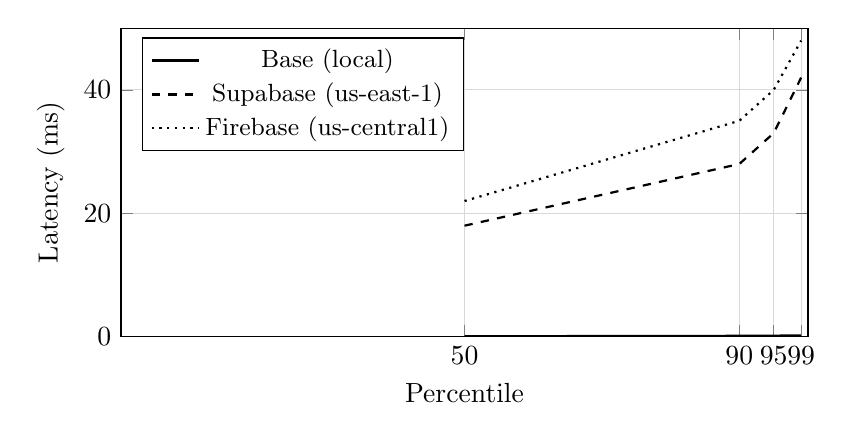
\begin{tikzpicture}
\begin{axis}[
    width=0.85\linewidth,
    height=5.5cm,
    xlabel={Percentile},
    ylabel={Latency (ms)},
    xmin=0, xmax=100,
    ymin=0, ymax=50,
    grid=major,
    grid style={gray!30},
    legend pos=north west,
    legend style={font=\small},
    xtick={50,90,95,99},
]
\addplot[thick, black, mark=none] coordinates {
    (50, 0.08) (90, 0.15) (95, 0.18) (99, 0.21)
};
\addlegendentry{Base (local)}
\addplot[thick, black, dashed, mark=none] coordinates {
    (50, 18) (90, 28) (95, 33) (99, 42)
};
\addlegendentry{Supabase (us-east-1)}
\addplot[thick, black, dotted, mark=none] coordinates {
    (50, 22) (90, 35) (95, 40) (99, 48)
};
\addlegendentry{Firebase (us-central1)}
\end{axis}
\end{tikzpicture}
\end{center}

This is not a benchmark of database engines. SQLite is not faster than
PostgreSQL for complex queries. This is a benchmark of architectures. A local
database will always beat a remote one for single-record operations because
physics imposes a floor on network latency that no optimization can remove.

% ============================================================================
\section{Production Deployment}
\label{sec:production}
% ============================================================================

Base has been in production at Hanzo since December 2022. Current deployment
statistics:

\begin{itemize}[leftmargin=1.1em]
    \item 2,800+ applications using Base as their primary backend.
    \item 1,200+ organizations across the Hanzo ecosystem.
    \item 40+ internal Hanzo applications (console, insights, commerce admin).
    \item Median p99 latency: 2.3~ms across all API operations.
    \item 99.97\% uptime over the trailing 12 months.
    \item Zero data loss incidents since launch.
\end{itemize}

\subsection{Migration from PocketBase}

Base maintains backward compatibility with PocketBase's API surface. Existing
PocketBase applications can migrate to Base by replacing the binary. The
migration path:

\begin{enumerate}[leftmargin=1.4em]
    \item Replace the PocketBase binary with the Base binary.
    \item Run \texttt{base migrate up} to apply schema additions (sqlcipher
    fields, sync metadata tables).
    \item Optionally enable sqlcipher encryption with \texttt{base encrypt}
    (re-encrypts the database in place).
    \item Optionally configure Hanzo IAM by setting the OIDC issuer URL.
\end{enumerate}

The existing SQLite database is preserved. No data export/import is required.

% ============================================================================
\section{Related Work}
\label{sec:related}
% ============================================================================

\paragraph{Local-first software.} Kleppmann et al.~\cite{kleppmann2019} define
local-first software as applications where the primary copy of data is on the
user's device. Base implements this vision with a production-grade runtime.
The key difference from academic CRDT systems (Automerge~\cite{automerge},
Yjs~\cite{yjs}) is that Base provides the full application stack---database,
auth, API, functions---not just a replication library.

\paragraph{CRDTs.} Shapiro et al.~\cite{shapiro2011crdt} formalize
conflict-free replicated data types. Base uses operation-based CRDTs with a
hybrid logical clock for causal ordering. The LWW register at field granularity
is a pragmatic choice that trades theoretical richness (counter CRDTs,
set CRDTs) for simplicity and predictability.

\paragraph{Encrypted databases.} CryptDB~\cite{cryptdb} and
Mylar~\cite{mylar} explore encryption in relational databases.
Base's approach is simpler: full-database encryption via sqlcipher plus
selective field-level encryption via KMS. This avoids the complexity of
onion encryption schemes while providing the practical guarantees that
applications need.

% ============================================================================
\section{Conclusion}
\label{sec:conclusion}
% ============================================================================

Base is not a backend framework. It is the runtime for sovereign applications.
The distinction matters. A framework assumes an environment---a cloud provider,
a database server, a container orchestrator. A runtime \emph{is} the
environment. Base carries its own database, its own auth, its own function
execution, its own sync protocol. It runs anywhere a Go binary runs.

The design principles are:

\begin{enumerate}[leftmargin=1.4em]
    \item \textbf{Local first}: The device is the source of truth. The network
    is an optimization, not a requirement.
    \item \textbf{Encrypted by default}: Data at rest is encrypted. Field-level
    encryption is available for sensitive data. Keys are user-controlled.
    \item \textbf{Sync, don't migrate}: CRDT-based replication means data flows
    between devices without schema migrations or conflict resolution dialogs.
    \item \textbf{Chain-optional}: Lux integration provides key policy,
    identity, and threshold controls for applications that need them. Those
    that do not need them pay no cost.
    \item \textbf{One binary}: No external dependencies. No infrastructure
    prerequisites. Download, run, build.
\end{enumerate}

The personal computer gave individuals sovereignty over computation. The
smartphone gave individuals sovereignty over communication. Base gives
individuals sovereignty over their data. That is the thesis. The 10,400
encrypted writes per second are just the proof.

% ============================================================================
% REFERENCES
% ============================================================================
\begin{thebibliography}{99}

\bibitem{hanzobase}
Z.~Kelling.
\newblock Hanzo Base: An open-source backend runtime with embedded database,
authentication, and {JavaScript} plugin system.
\newblock \emph{Hanzo AI Research}, December 2022.

\bibitem{luxwhitepaper}
{Lux Partners}.
\newblock Lux: A scalable multi-consensus blockchain with post-quantum
cryptography.
\newblock \emph{Lux Network Technical Report}, 2024.

\bibitem{luxtrust}
Z.~Kelling.
\newblock The Lux Trust Kernel: Threshold cryptography for decentralized key
management.
\newblock \emph{Lux Network Technical Report}, 2025.

\bibitem{luxapp}
Z.~Kelling.
\newblock Lux Application Architecture: Sovereign applications on
multi-consensus infrastructure.
\newblock \emph{Lux Network Technical Report}, 2025.

\bibitem{hanzoplatform}
M.~Chen, D.~Wei, and Z.~Kelling.
\newblock Hanzo Platform: {PaaS} for {AI}-native application deployment.
\newblock \emph{Hanzo AI Research}, December 2021.

\bibitem{kleppmann2019}
M.~Kleppmann, A.~Wiggins, P.~van Hardenberg, and M.~McGranaghan.
\newblock Local-first software: You own your data, in spite of the cloud.
\newblock In \emph{Onward!}, ACM, 2019.

\bibitem{automerge}
M.~Kleppmann and A.~R.~Beresford.
\newblock A conflict-free replicated {JSON} datatype.
\newblock \emph{IEEE TPDS}, 28(10):2733--2746, 2017.

\bibitem{yjs}
K.~Jahns.
\newblock Yjs: A {CRDT} framework for shared editing.
\newblock \url{https://github.com/yjs/yjs}, 2019.

\bibitem{kulkarni2014hlc}
S.~Kulkarni, M.~Demirbas, D.~Madeppa, B.~Avva, and M.~Leone.
\newblock Logical physical clocks and consistent snapshots in globally
distributed databases.
\newblock In \emph{OPODIS}, 2014.

\bibitem{shapiro2011crdt}
M.~Shapiro, N.~Pregui\c{c}a, C.~Baquero, and M.~Zawirski.
\newblock Conflict-free replicated data types.
\newblock In \emph{SSS}, Springer, 2011.

\bibitem{cryptdb}
R.~A.~Popa, C.~M.~S.~Redfield, N.~Zeldovich, and H.~Balakrishnan.
\newblock {CryptDB}: Protecting confidentiality with encrypted query processing.
\newblock In \emph{SOSP}, ACM, 2011.

\bibitem{mylar}
R.~A.~Popa, E.~Stark, J.~Helfer, S.~Valdez, N.~Zeldovich,
M.~F.~Kaashoek, and H.~Balakrishnan.
\newblock Building web applications on top of encrypted data using {Mylar}.
\newblock In \emph{NSDI}, USENIX, 2014.

\bibitem{pocketbase2022}
G.~Kostadinov.
\newblock {PocketBase}: Open-source backend in 1 file.
\newblock \url{https://pocketbase.io}, 2022.

\end{thebibliography}

\end{document}
